\section{\review{Dodecapolar RDT}}

% Fill 9339
% https://logbook.cern.ch/elogbook-server#/logbook?logbookId=1081&dateFrom=2024-03-10T00%3A00%3A00&dateTo=2024-03-11T00%3A00%3A00
% http://localhost:8888/lab/workspaces/auto-Z/tree/work_afs2/jupyter/resonance_driving_terms/simulations/first_dodecapole_rdt/Plots.ipynb

During the commissioning of 2024, resonance driving terms measurements were performed by kicking the
beam at various strengths with the AC-Dipole at injection energy. Those measurements were intended
to measure several RDTs with a focus on decapoles and their associated corrections. Kicks 
were performed using the nominal settings for octupolar and decapolar correctors, first with $Q''$
corrections and then with additional $Q''$ corrections applied.
A distinct line in the vertical spectrum was observed at $5Q_y$, as shows
\cref{fig:high_orders:spectrum_dodecapole_5qy}. This line is contributed to by dodecapolar fields
(see \cref{appendix:rdts}) and is proportional to the vertical oscillation amplitude.

\begin{figure}[!htb]
    \centering
    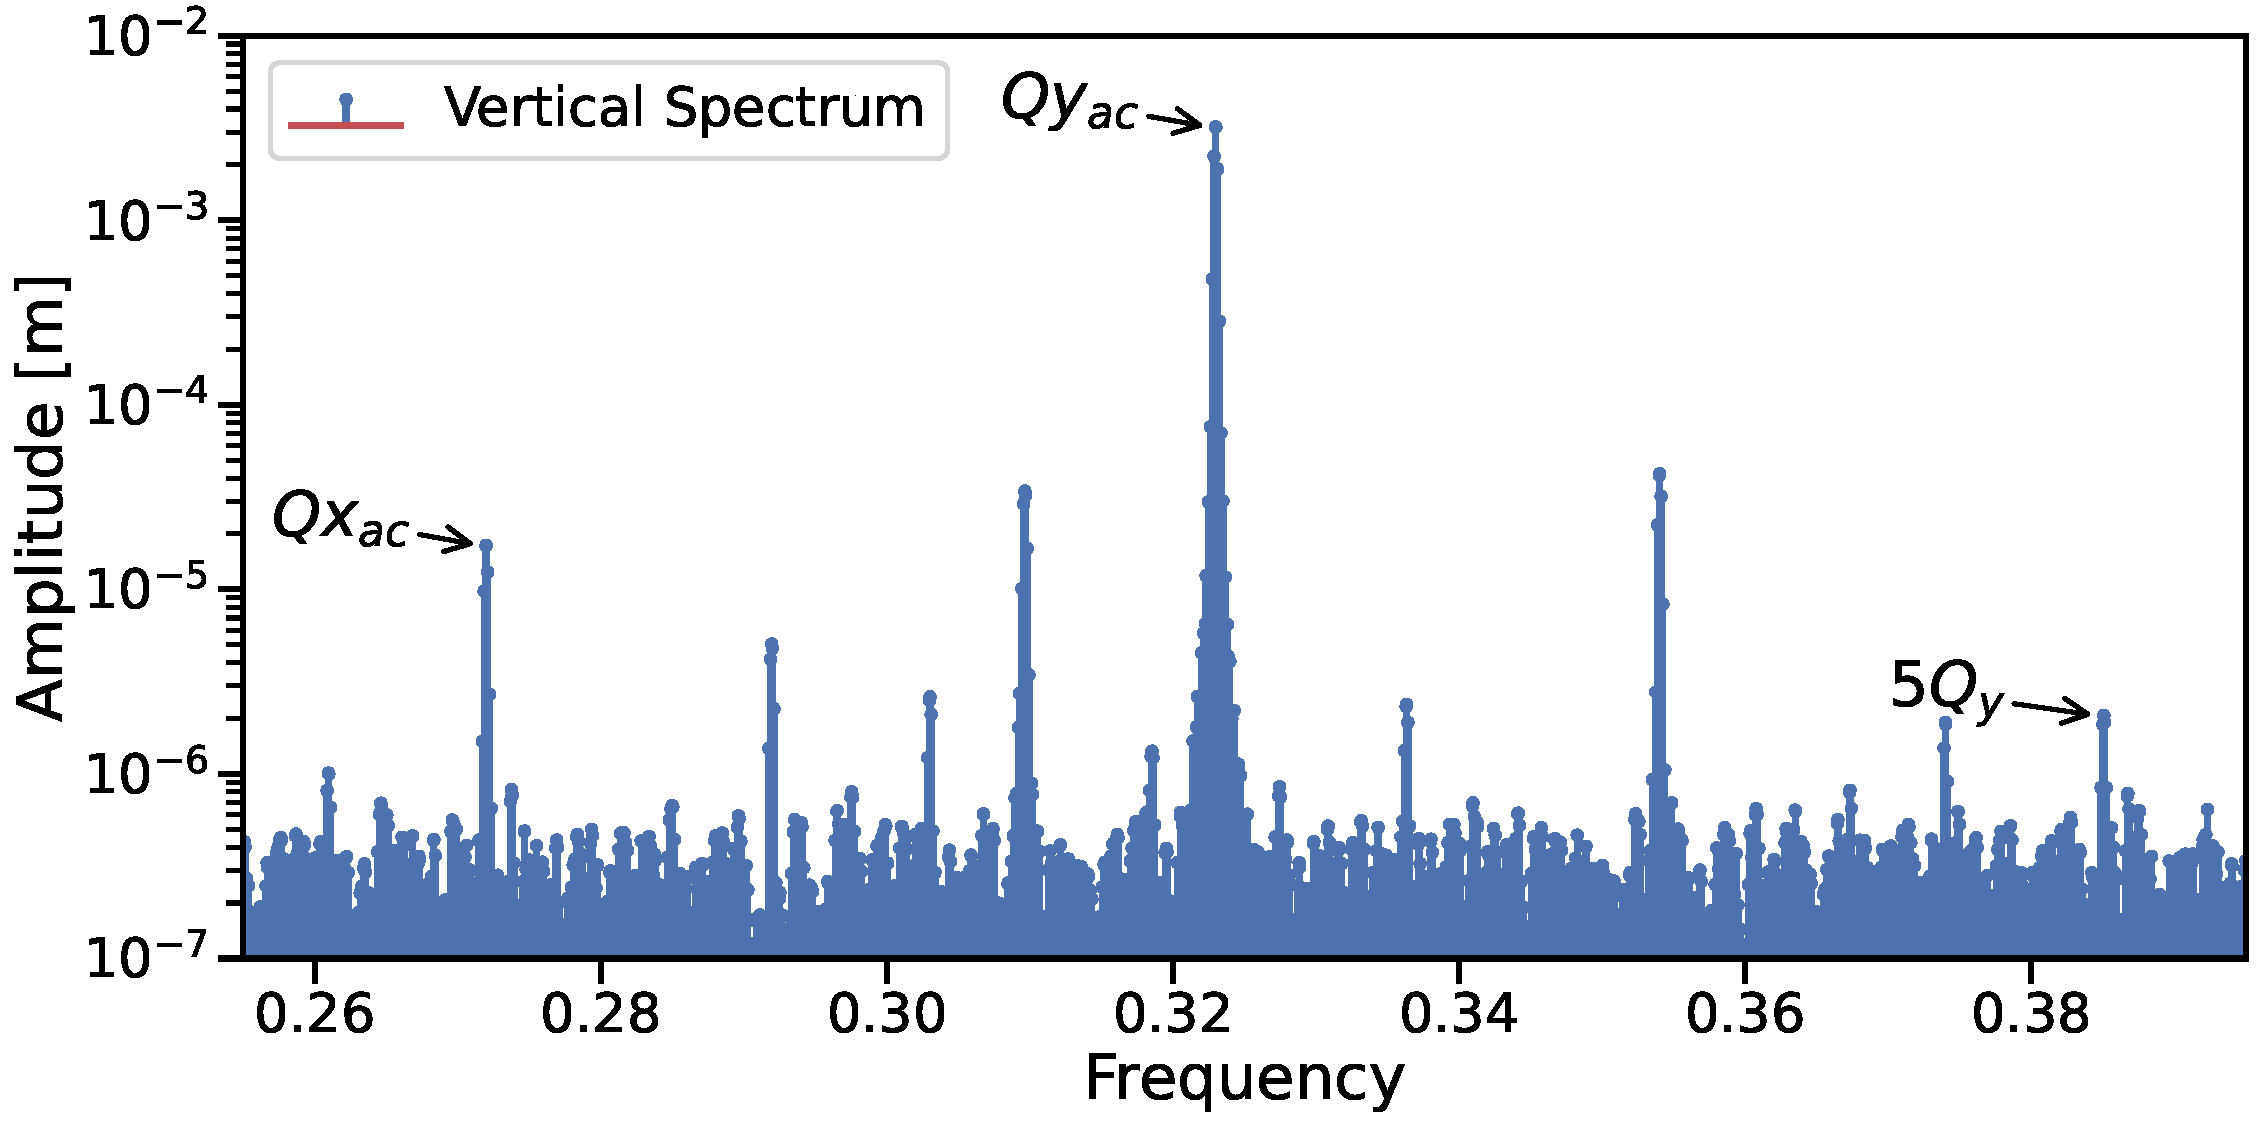
\includegraphics[width=0.8\textwidth]{./images/spectrum_dodecapole_5qy.pdf}
    \caption{Vertical spectrum of recorded turn-by-turn data for Beam 1 showing the tunes driven by the
    AC-Dipole along with a line contributed to by dodecapolar fields.}
    \label{fig:high_orders:spectrum_dodecapole_5qy}
\end{figure}

To achieve these measurements, the kick strength of the AC-Dipole was set up to $40\%$ of its
maximum, made possible by the newly introduced collimator sequence. The specific excited resonance
of the observed line is the $6Q_y$, related to the RDT $f_{0060}$.
\Cref{fig:high_orders:dodecapolar_f0060} highlights the real part of this RDT taken with nominal
corrections and the repeatability of the measurement at varying kick strengths. The RMS of the
amplitude of these kicks is of $3.5\cdot10^8$

\begin{figure}[!htb]
    \centering
    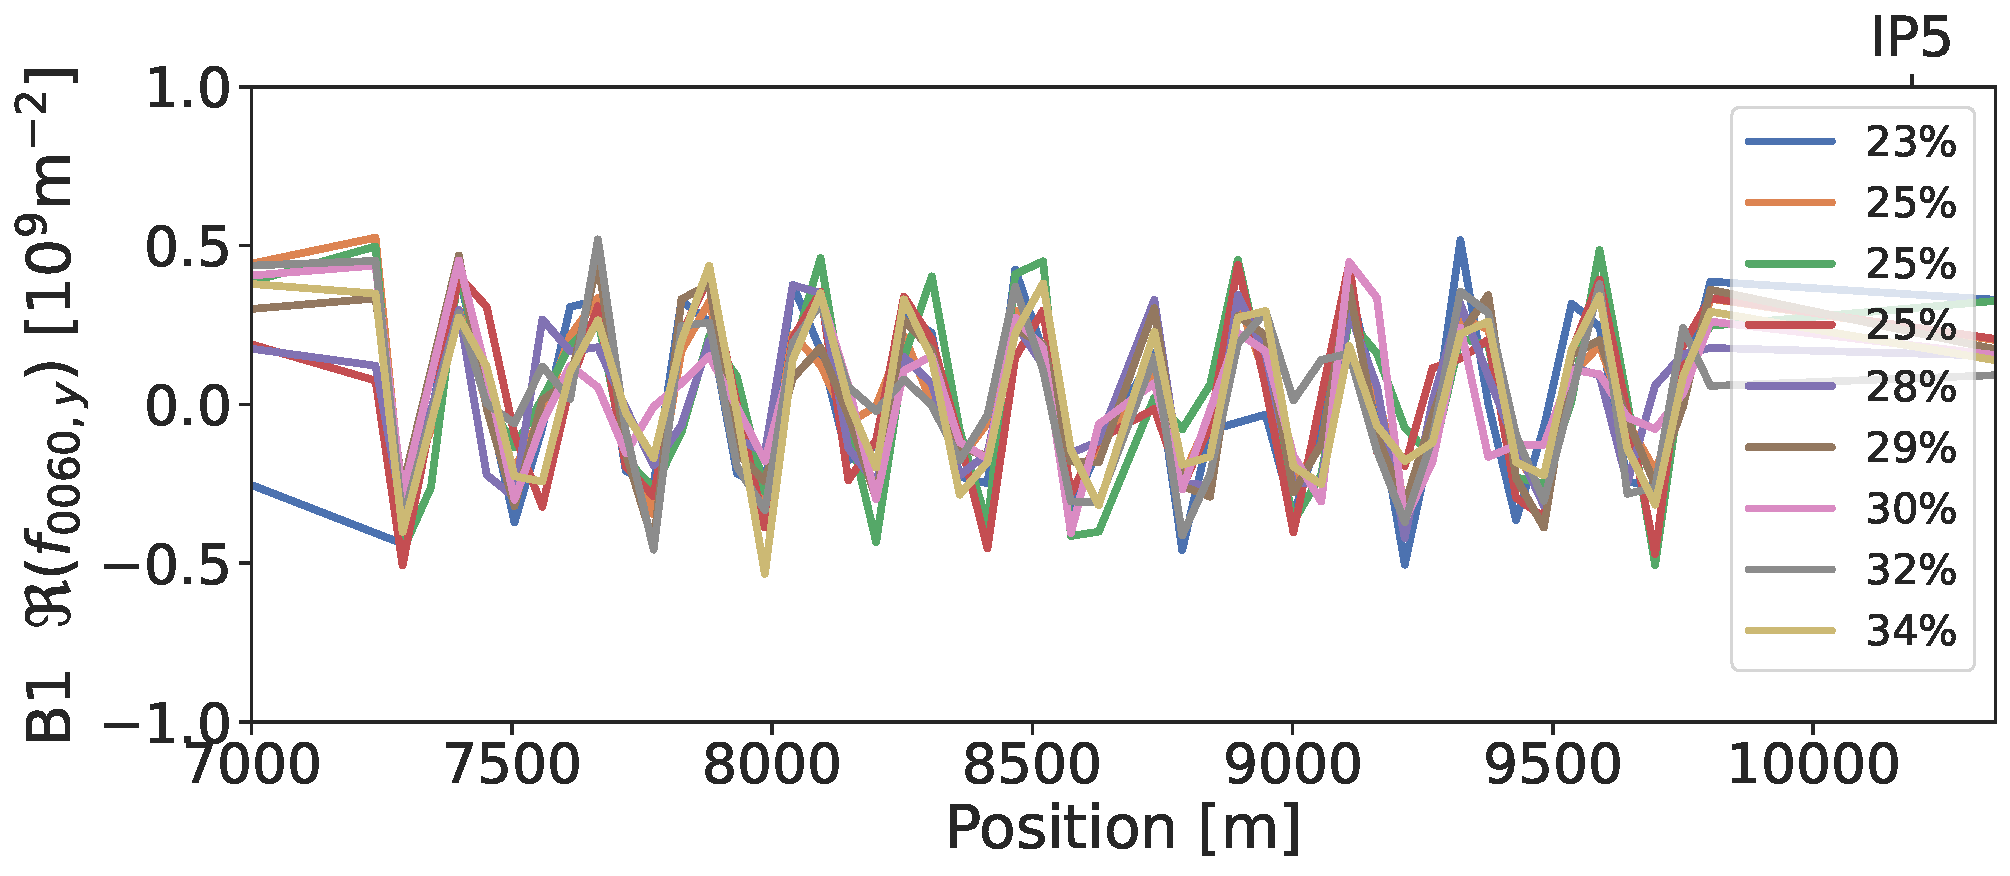
\includegraphics[width=0.8\textwidth]{./images/f0060y_all_meas_real.pdf}
    \caption{Real part of the dodecapolar RDT $f_{0060}$ measured with several kick strengths. The
    RMS amplitude is of $3.5\cdot10^{8}$.}
    \label{fig:high_orders:dodecapolar_f0060}
\end{figure}

Similar to the decapoles discussed in \cref{section:decapoles:feed_up}, the dodecapolar RDTs can be
influenced by lower-order components, as shown in
\cref{table:appendix:transfer_maps:bch_resulting_orders_combination}. At the second-order BCH, a
combination of sextupoles and decapoles, as well as a combination of octupoles, generate a
decapolar-like field. At the third and fourth orders, these fields are respectively generated by a
combination of sextupoles with octupoles and by sextupoles.
Several tracking simulations were performed with various combinations of field errors, ranging from
normal and skew sextupoles ($a,b_3$) to decaoctupoles ($a,b_9$), including as well coupling.
Beta-beating is not included as $b_2$ errors also have an effect on the phase.
\Cref{fig:high_orders:simulations_f0060} shows the RMS amplitude of the RDT $f_{0060}$ for each of
these simulations. As expected from the analytical equations, the lower-order multipoles do
contribute to this RDT and seem to cancel the $b_6$ component. It is though apparent that Beam 1 and
Beam 2 do not have the same contributions from the dodecapolar errors. These seem to be compensated
by other field errors for Beam 1.

\begin{figure}[H]
    \centering
    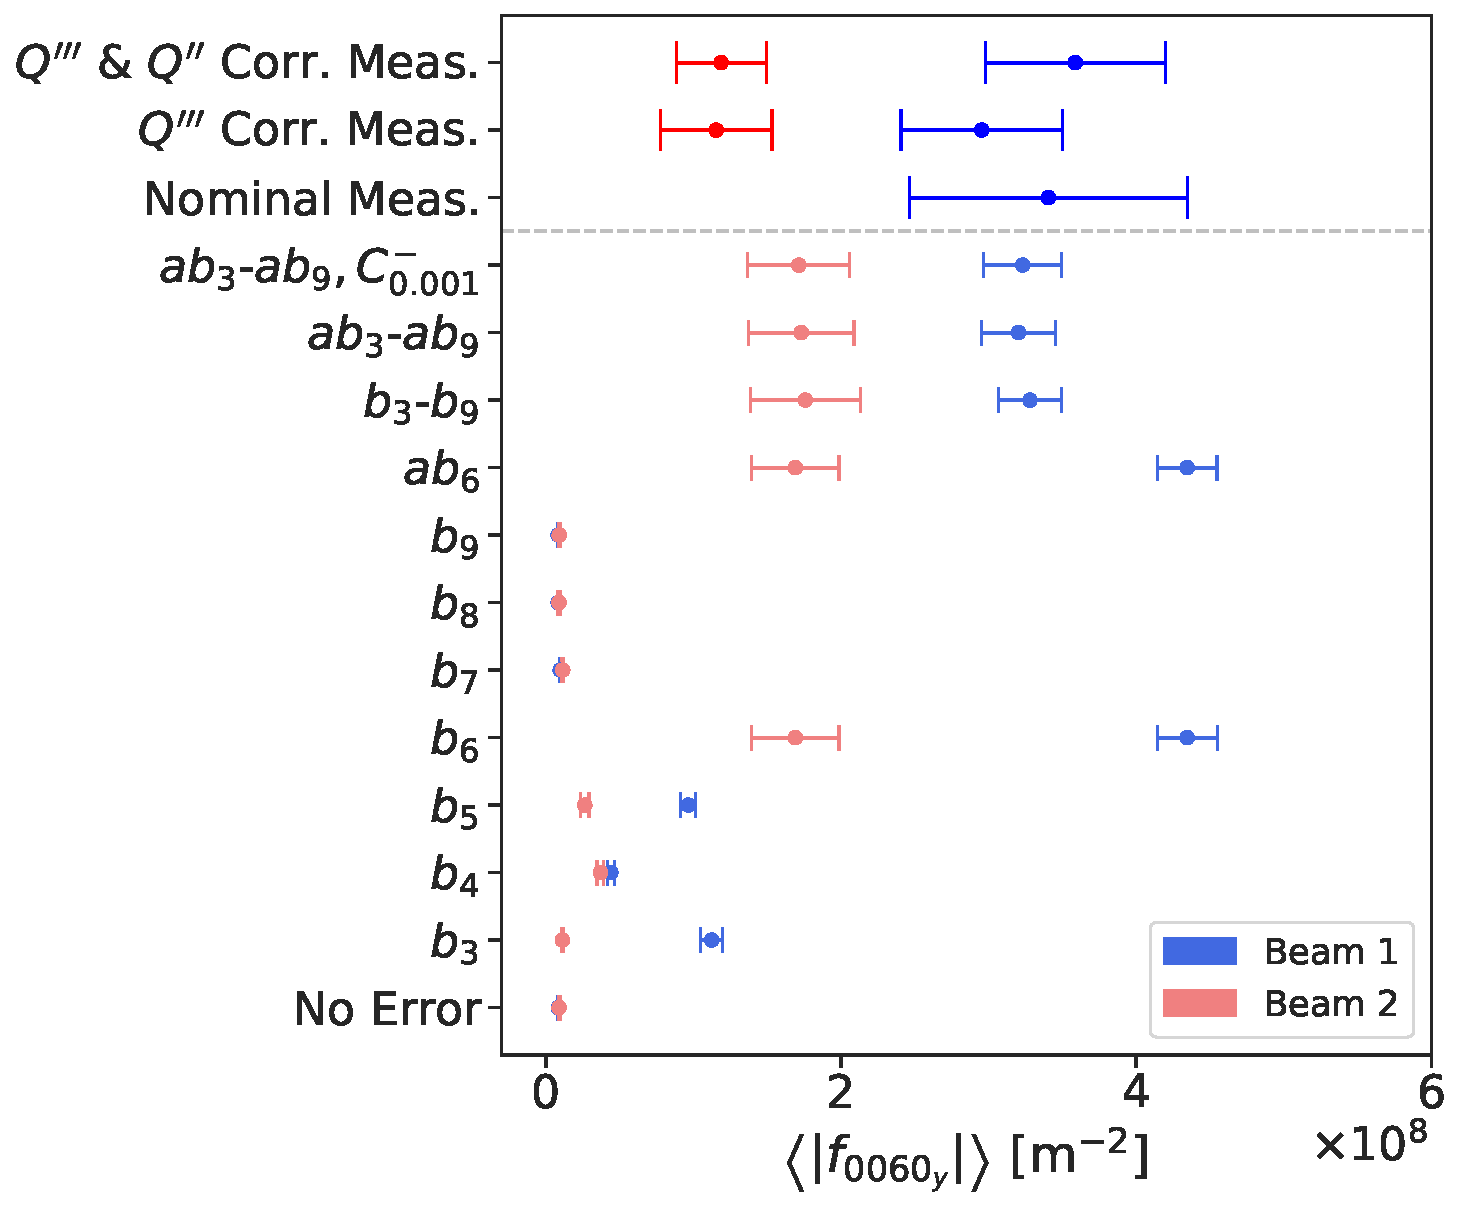
\includegraphics[width=0.7\textwidth]{./images/simulations_f0060.pdf}
    \caption{Measured and simulated RDT $f_{0060}$ with various normal and skew field errors.
    Coupling is set to a common value seen in operation.}
    \label{fig:high_orders:simulations_f0060}
\end{figure}

The previously referenced measurements are also compared to these simulations. The measurement for
Beam 2 with the nominal corrections could not be reliably exploited and is not included.  The RDTs
from these measurements are similar in amplitude, despite the different configurations for the
octupolar and decapolar correctors. This suggests that, at these strength variations, the high-order
correctors do not significantly affect the dodecapolar RDT $f_{0060}$. It is however important to
note that predicting the contributions from lower-order multipoles remains difficult.